\begin{figure*}[t]
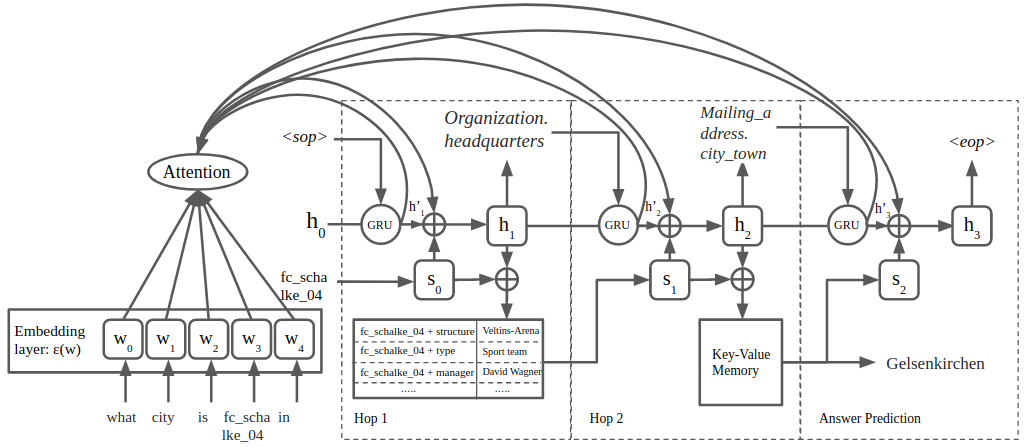
\includegraphics[width=2.1\columnwidth]{figs/model2.png}
\caption{\fontsize{10}{12}\selectfont An illustration of how our model answers the question "What city is fc\_schalke\_04 in?". The entity linker extracts \textit{fc\_schalke\_04} as the topic entity. $[\textit{\textless sop\textgreater}, \textit{Organization.headquarters} , \textit{Mailing\_address.city\_town, \textless eop\textgreater}]$ is the predicted relation path \cheng{Shall we include entities in the middle in the path? Are sop and eop defined already?} and \textit{Gelesenkirchen} is the predicted answer. The symbol $\bigoplus$ represents concatenation. }
\label{fig:model}
\end{figure*}


\section{Model}
 Given a question $q$ and its topic entity $e_0$ (identified by entity linking \cheng{Did we mention entity linking before?}), our model aims to find the reasoning path $\mathbf{r} = (e_{0},r_{1},e_{1},r_{2}, \cdots,e_{T-1}, r_{T})$ and the answer $y$ from the knowledge base $\mathcal{KB}$. In this section, we first present the design of our model architecture, and then explain the training and inference algorithms in detail.  

\subsection{Model Architecture}


Figure \ref{fig:model} illustrates the architecture of our model. Our base model is similar to a RNN structure.

\subsubsection{Question Encoding} All the words $w_0,w_1,\cdots,w_{|q|-1}$ in the given question $q$ are first sent to a fixed embedding layer to acquire word embeddings $\varepsilon(w_0),\varepsilon(w_1),\cdots,\varepsilon(w_{|q|-1})$. \cheng{Does the symbol match the one in diagram?} To reduce computational cost, the embedding layer is pre-trained and not updated during RNN training. Because we wish to learn different question context representations to show different reasoning focus at each hop, the  word embeddings are combined in different ways to form the question embedding  based on attention weights learned by relation prediction module at each hop.
% $\varepsilon(\cdot)$ function represents gathering embedding of the input from the corresponding pre-trained embeddings matrix. 



%\subsubsection{Reasoning Decoding} The decoding module consists of relation prediction module and entity prediction module.

\subsubsection{Relation Prediction} \cheng{What do you mean by prediction}
We model relation prediction as a sequence prediction task using recurrent neural network with gated recurrent units (GRU). The hidden representations of GRU unit and predicted relation at timestep $t$ are denoted by $h_t$ and $r_t$ respectively. At timestep $t$, the model relies on the attention mechanism~\cite{DBLP:journals/corr/BahdanauCB14} to produce a question context vector $c_t$. Specifically we first apply GRU to produce a temporary hidden state  $h_{t}'=GRU(h_{t-1}, r_{t-1})$, and then apply a parameterized feed-forward neural network $a$ to calculate the similarity score $u_{tk} = a(h'_{t},\varepsilon(w_k))$ of two inputs $h'_{t}$ and $\varepsilon(w_k)$,  and then these scores are normalized into attention weights $\alpha_{tk}=\frac{\exp (u_{tk})}{\sum_{0\leq j\leq |q|-1}\exp (u_{tj})}$, which are used to produce the question context vector $c_t=\sum_{0\leq j\leq |q|-1}\alpha_{tj}\varepsilon(w_j)$. \cheng{Should this be put in the question encoding section?}
% \begin{align}
% h'_{t} = GRU(h_{t-1}, r_{t-1}) 
% \end{align}
% \vspace{-3ex}
% \begin{align}
% u_{tk} = a(h'_{t},\varepsilon(w_k))
% \end{align}
% \vspace{-3ex}
% \begin{align}
% \alpha_{tk} = \frac{\exp (u_{tk})}{\sum_{0\leq j\leq |q|-1}\exp (u_{tj})}
% \end{align}
% \vspace{-1ex}
% %\[\alpha_{tk} = \frac{u_{tk}}{\sum_{j}u_{tj}}\]
% \begin{align}
% c_t = \sum_{0\leq j\leq |q|-1}\alpha_{tj}\varepsilon(w_j)
% \end{align}

 %After having all above computations done, 

The model then concatenates temporary hidden state $h_{t}'$, entity representation $\varepsilon(e_{t-1})$, and question context $c_t$ together, and pass the concatenation through a linear transformation $f$ with ReLU activation. The process can be  written as:
\begin{align}
h_t = ReLU(f([h'_{t}; \varepsilon(e_{t-1}); c_t]))
\end{align}

The probability of predicting the $j$-th relation in $\mathcal{R}$ at timestep $t$ is

\begin{align}
o^j_t = \frac{\exp <h_t,\varepsilon(r_j)>}{\sum_k\exp <h_t,\varepsilon(r_k)>}
\label{eq:r_prob}
\end{align}

where $\varepsilon$ is the embedding  function, $<>$ is the dot product between two inputs. 

After the model predicts a relation $r_t$, \cheng{What do you mean by predicting a relation?} it can simply execute a query $(e_{t-1}, r_{t-1}, ?e_t)$ on knowledge base to get an entity $e_t$ from the knowledge base, and feed it to next timestep. Another way to collect this entity is via a soft lookup with a key-value memory network structure. We provide more details in the appendix.


\subsubsection{Objective Functions}

The model can be trained in two ways: to maximize the joint probability $P(y,\mathbf{r}|q,\mathcal{KB})$, or to maximize answer probability $P(y|q,\mathcal{KB})$ directly by marginalizing out relation paths $\mathbf{r}$. The former one was adopted by many existing KBQA papers \cite{DBLP:conf/coling/ZhouHZ18}, while the later is novel to KBQA task. We now describe our objective in detail. Without loss of generality, we will omit $\mathcal{KB}$ in these formulas.

At a timestep $t$, previous relations and entities consist the current reasoning path $\mathbf{r_t} = (e_{0},r_{1},e_{1},r_{2}, \cdots,e_{t-1})$. Our model first predict a relation $r_t$ from the set of relation candidates $\mathcal{R}$:
\begin{align}
P(r_t|q,\mathbf{r_t}) = \sum_{j=1}^{\mathcal{R}}\hat{o}^j_t{o^j_t}
\end{align}
Given the predicted $r_t$ and the previous entity $e_{t-1}$, we can get a set of entities $e_t$ based on knowledge base lookup. We define the number of founded $e_t$ as $|e_t|$. Then we can define the probability of generating an entity $e_t$ given a relation path $\mathbf{r}$ as: \kechen{add some explanations that we why define in this way. and polish english}
\begin{align}
P(e|\mathbf{r},q) = 1/|e_t|
\end{align}
Finally, our training goal is to maximize the probability of generating the correct answer, and the training objective can be written as:

\begin{equation}
\begin{aligned}
\mathcal{L} &= -\log P(y|q) \\
            &= -\log(\sum_{\mathbf{r}\in \mathcal{P}} P(y|\mathbf{r},q)\sum_{t=1}^T P(r|\mathbf{r},q)P(e|\mathbf{r},q))\\
            &= -\log(\sum_{\mathbf{r}\in \mathcal{P}} \sum_{t=1}^T\sum_{j=1}^{\mathcal{R}}\hat{o}^j_t{o^j_t} 1/|e_t|)
\end{aligned}
\label{obj:latent}
\end{equation}


%To further improve the diversity of the outputs, we follow \newcite{}'s idea to optimize mutual information instead of log likelihood. Specifically, we observe that 


\subsection{Training and Inference}
\kechen{merge 2.2 to 2.1.3 and create new 2.2 only for training algorithm? should we keep join objective here?}





\subsubsection{Joint probability objective} This objective consists of two loss terms for prediction of relations and prediction of answer respectively. The loss on one instance is defined as follows:
\begin{align}
 \mathcal{L} = \sum_{h}\mathcal{L}_r^{h} + \mathcal{L}_e 
 \end{align}
  \vspace{-3ex}
\begin{align}
 \mathcal{L}_r^{h} = -\sum_{j=1}^{\mathcal{R}}\hat{o}^h_j\log{o^h_j},\;\;\mathcal{L}_e = -\sum_{i=1}^{\mathcal{E}}\hat{g}_i\log{g_i}
\end{align}
where $\mathcal{L}_e$ and $\mathcal{L}_r$ denote the cross entropy errors. $\hat{o}^h_j$ and $o^h_j$ represent gold distribution (one-hot representation) and predicted distribution defined by Eq. \ref{eq:r_prob} over relations at hop $h$. $\hat{g}_i$ and $g^h_i$ represent gold distribution and predicted distribution defined by Eq. \ref{eq:e_prob} over entities. Minimizing the sum of these two loss terms can be easily transformed to maximizing the joint probability of answer and the relation path:
\begin{equation}
\begin{aligned}
\mathcal{L} &= -\log P(y|\mathbf{r},q) - \log P(\mathbf{r}|q) \\
            &= -\log P(y,\mathbf{r}|q)
\end{aligned}
\end{equation}

For each QA pair, the joint objective function pushes the model to allocate all of the probability mass to the given relation path. However, this assumption does not reflect real-world reasoning procedures: Figure \ref{QAPaths} shows there could be multiple relation paths for one QA sample. 
To overcome this issue, some propose to use each relation path to construct a training instance, and the objective on one QA sample becomes \kechen{how to write prob of multiple e?}:
\begin{align}
\mathcal{L} = -\sum_{\mathbf{r}\in \mathcal{P}}\log P(y,\mathbf{r}|q)
\end{align}

where $\mathcal{P}$ is the set of relation paths of one QA sample labeled in training set. Although this objective has ability to learn from multiple relation paths, it is limited to fit the training data, which means only the labeled relation paths are considered.
 % It is not easy to enumerate all relation path with human labeling. 
 In addition, this objective has an undesired consequence in practical model training: because of the multiplication operation, the model has to assign equally high probabilities to all given relation paths in order to maximize the product of the probabilities. If only some relation paths receive high probabilities while others receive low probabilities, the production will still be low. As a consequence, the model cannot differentiate bad relation paths from good ones by assigning different probabilities to them.

\subsubsection{Marginal probability objective} We propose a new way to train KBQA model by treating relation path as latent variable, and marginalize it out to maximize the final answer probability directly:
\begin{equation}
\begin{aligned}
\mathcal{L} &=  -\log(\sum_{\mathbf{r}\in \mathcal{P}}( P(y|\mathbf{r},q)P(\mathbf{r}|q))\\
            &= -\log P(y|q)
\end{aligned}
\label{obj:latent}
\end{equation}

With our proposed training objective, in which the multiplication operation is replaced by the summation operation, it suffices to concentrate only on reasonable reasoning paths for each QA pair. Using Jensen's inequality, one can show that this marginal probability objective maximize the answer probability directly which is the learning goal of KBQA task, while joint probability objective maximizes a lower bound. Also, one can easily prove that the above objective pushes the model to assign both high or low probabilities for $P(y|\mathbf{r},q)$ and $P(\mathbf{r}|q)$. That is, a good relation path (high probability to point to the correct answer) also gets a high probability allocation. %A benefit of using our model with this objective is that the key hashing process filters out irrelevant memory slots from the full search space. During training, the smaller relation paths that point to an answer set, the larger probability mass will be assigned to this relation path. %This feature satisfies our definition of good path in the introduction. 


Training this objective requires summing up all valid relation paths from the topic entity to the answer entity in the knowledge base. Thus evaluating this objective exactly can be intractable. As we showed in the early example, some relation paths ($R_5, R_6, R_7$ in Figure \ref{QAPaths}) are not very helpful to training \kechen{P(y|R567) is very small in the marginalization}, and thus should be removed from training or assigned low probabilities. To achieve this goal, we first apply depth first search (DFS) algorithm with maximize 3 hops to get valid path candidates. The algorithm starts traversal from the topic entity node and ends at the answer entity node. All possible paths between the topic entity and the answer entity within 3 hops are extracted as candidates. We then set a threshold to remove paths which point to too many entities at the last hop. To further filter out bad relation paths, we propose to dynamically choose relation paths deemed as most probable by the current model during training. The overall training procedure is summarized in Algorithm \ref{alg:train}. Note that training with this algorithm does not require ground truth relation path label. Labeled relation path can be seen as plus, but not necessary. If it is given, we can either replace $\mathcal{P}$ with ground truth relation set, or train the model with joint probability objective using ground truth label first and transit to marginal probability objective after a few epochs.

\begin{algorithm}
  \SetKwInOut{Input}{Input}
  \SetKwInOut{Output}{Output}

 % \underline{function Euclid} $(a,b)$\;
  \Input{KBQA dataset $(q^{(n)},y^{(n)}, e_0^{(n)}),n=1,2,\cdots,N$, \\
  Knowledge Base $\mathcal{KB}$, \\
  Threshold $k_1$ and $k_2$. }
  \Output{Trained model parameters}
  Use DFS algorithm to get a set of paths $\mathcal{P}$ from $e_0^{(n)}$ to $y^{(n)}$.\\
  Remove paths that point to more than $k_1$ entities from $\mathcal{P}$.\\
  % Initialize model parameters\\
  \ForEach {batch}{
    % \ForEach {batch }{
      \ForEach{$(x^{n},\mathbf{y}^{n})$ in the batch}{
        Get top $k_2$ paths of $\mathcal{P}$ sorted by $P(\mathbf{r}|q)$ :\\
		  	$\{{\mathbf{r}}^n_{1},\cdots,{\mathbf{r}}^n_{k_2}, P({\mathbf{r}}^n_{1}|q^n),\cdots,P({\mathbf{r}}^n_{K}|q^n,$ $P({y}^n_{1}|{\mathbf{r}}^n_{1},q^n),\cdots,P({y}^n_{K}|{\mathbf{r}}^n_{n},q^n)\}$ \hspace{4ex}= Inference\_with\_current\_model$(q^{n},\mathcal{P}$)\\
		  	$\mathcal{P} = \{{\mathbf{r}}^n_{1},\cdots,{\mathbf{r}}^n_{k_2} \}$\\
        }  
              Update model parameters by maximizing $\sum\limits_{(q^{n},{y}^{n}) \in \text{batch}} \log \sum\limits_{\mathbf{r} \in \mathcal{P}}  P(y^{n}|\mathbf{r},q^{n}) P(\mathbf{r}|q^{n}) $
        }


    % }
  \caption{Training method for our model}
  \label{alg:train}
\end{algorithm}
\subsubsection{Inference} We adopt beam search to predict the relation path and use knowledge base lookup to predict the answer. Different from the vanilla beam search that allows to search on the full set of relations $\mathcal{R}$. We add two constraints to beam search so as to only select the valid path based on the knowledge base. (1) The first relation should get connected with the topic entity. (2) Each relation should get connected with the previous relation where uses an entity as the bridge. We then use an ensemble strategy to re-rank the searching results. Formally, given beam search outputs $\mathbf{r}_{1},\cdots,\mathbf{r}_{b}$ and $P(\mathbf{r}_{1}),\cdots,P(\mathbf{r}_{b})$, our model first use knowledge base lookup to get a list of different answer sets $\hat{y}_1,\cdots,\hat{y}_m$, where $m$ is the number of answer sets generated by $b$ relation paths, hence $m \leq b$. We then take the sum of the probabilities of relation paths $\mathbf{r}_i$ leading to the same predicted answer set and compare these sums. The final selected answer set $\hat{y}$ is the one with the maximum sum value. To represent it mathematically:
\begin{equation}
\hat{y}=\argmax_{\hat{y}_l} \sum_{i} P(\mathbf{r}_i\rightarrow \hat{y}_l)
\end{equation}
where $P(\mathbf{r}_i\rightarrow \hat{y}_l)$ is the probability of a relation path leading to the predicted answer set $\hat{y}_l$ and $l \in \lbrace 1, \cdots, m\rbrace$.